\documentclass[tikz,border=8pt]{standalone}
% Shared look for every TikZ diagram. Load with % Shared look for every TikZ diagram. Load with % Shared look for every TikZ diagram. Load with \input{../../tools/tikz-style.tex}
\usepackage[T1]{fontenc}
\usepackage{lmodern}
\renewcommand{\sfdefault}{lmr}  % diagrams use the same serif as the text
\usetikzlibrary{arrows.meta, positioning, shapes.geometric, calc, fit, backgrounds}
\definecolor{cblue}{HTML}{4C78A8}
\definecolor{corange}{HTML}{F58518}
\definecolor{cgreen}{HTML}{54A24B}
\definecolor{cred}{HTML}{E45756}
\definecolor{cpurple}{HTML}{B279A2}
\definecolor{cgrey}{HTML}{6B6B6B}
\tikzset{
  every picture/.style={font=\sffamily, line width=1.2pt},
  box/.style={draw=#1, fill=#1!12, rounded corners=4pt, align=center, inner sep=7pt, minimum height=1.1cm},
  box/.default=cgrey,
  arrow/.style={-{Stealth[length=3mm]}, draw=cgrey, line width=1.4pt},
  title/.style={font=\sffamily\bfseries\Large},
  note/.style={font=\sffamily\small, text=cgrey, align=center},
}
\AtBeginDocument{\hyphenpenalty=10000 \exhyphenpenalty=10000}

\usepackage[T1]{fontenc}
\usepackage{lmodern}
\renewcommand{\sfdefault}{lmr}  % diagrams use the same serif as the text
\usetikzlibrary{arrows.meta, positioning, shapes.geometric, calc, fit, backgrounds}
\definecolor{cblue}{HTML}{4C78A8}
\definecolor{corange}{HTML}{F58518}
\definecolor{cgreen}{HTML}{54A24B}
\definecolor{cred}{HTML}{E45756}
\definecolor{cpurple}{HTML}{B279A2}
\definecolor{cgrey}{HTML}{6B6B6B}
\tikzset{
  every picture/.style={font=\sffamily, line width=1.2pt},
  box/.style={draw=#1, fill=#1!12, rounded corners=4pt, align=center, inner sep=7pt, minimum height=1.1cm},
  box/.default=cgrey,
  arrow/.style={-{Stealth[length=3mm]}, draw=cgrey, line width=1.4pt},
  title/.style={font=\sffamily\bfseries\Large},
  note/.style={font=\sffamily\small, text=cgrey, align=center},
}
\AtBeginDocument{\hyphenpenalty=10000 \exhyphenpenalty=10000}

\usepackage[T1]{fontenc}
\usepackage{lmodern}
\renewcommand{\sfdefault}{lmr}  % diagrams use the same serif as the text
\usetikzlibrary{arrows.meta, positioning, shapes.geometric, calc, fit, backgrounds}
\definecolor{cblue}{HTML}{4C78A8}
\definecolor{corange}{HTML}{F58518}
\definecolor{cgreen}{HTML}{54A24B}
\definecolor{cred}{HTML}{E45756}
\definecolor{cpurple}{HTML}{B279A2}
\definecolor{cgrey}{HTML}{6B6B6B}
\tikzset{
  every picture/.style={font=\sffamily, line width=1.2pt},
  box/.style={draw=#1, fill=#1!12, rounded corners=4pt, align=center, inner sep=7pt, minimum height=1.1cm},
  box/.default=cgrey,
  arrow/.style={-{Stealth[length=3mm]}, draw=cgrey, line width=1.4pt},
  title/.style={font=\sffamily\bfseries\Large},
  note/.style={font=\sffamily\small, text=cgrey, align=center},
}
\AtBeginDocument{\hyphenpenalty=10000 \exhyphenpenalty=10000}

\newcommand{\cm}{\textcolor{corange}{\textbf{,}}}
\begin{document}
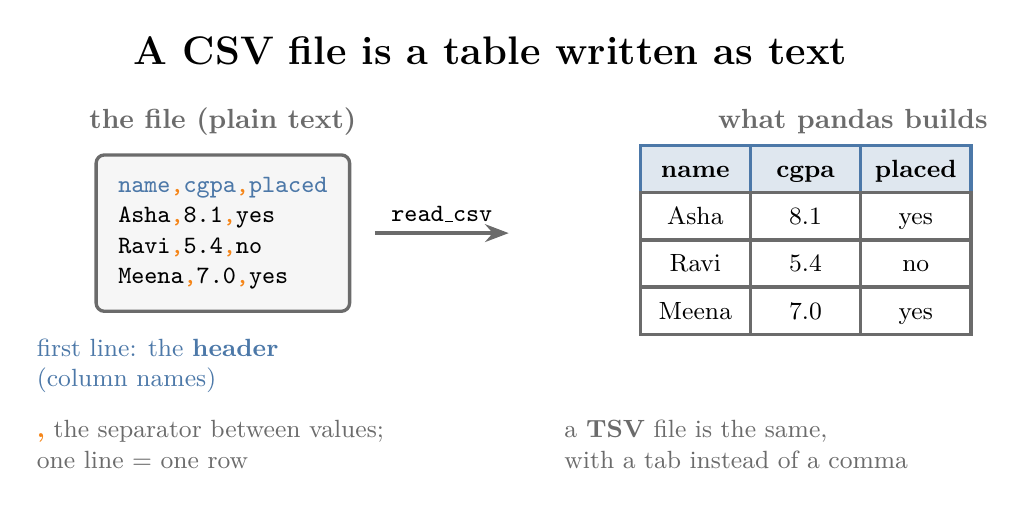
\begin{tikzpicture}
  \node[title] at (4.0,3.4) {A CSV file is a table written as text};
  % left: the raw text file
  \node[font=\bfseries, text=cgrey] at (0.6,2.5) {the file (plain text)};
  \node[draw=cgrey, fill=cgrey!6, rounded corners=3pt, align=left, inner sep=8pt, font=\ttfamily\small, anchor=north] (txt) at (0.6,2.1)
    {\textcolor{cblue}{\textbf{name\cm cgpa\cm placed}}\\ Asha\cm 8.1\cm yes\\ Ravi\cm 5.4\cm no\\ Meena\cm 7.0\cm yes};
  % right: the table
  \node[font=\bfseries, text=cgrey] at (8.6,2.5) {what pandas builds};
  \begin{scope}[shift={(6.6,1.9)}, font=\small]
    \foreach \c [count=\i from 0] in {name,cgpa,placed}
      \node[draw=cblue, fill=cblue!18, minimum width=1.4cm, minimum height=0.6cm, text height=1.8ex, text depth=0.4ex, font=\small\bfseries] at (\i*1.4,0) {\c};
    \foreach \a/\b/\c [count=\r] in {Asha/8.1/yes, Ravi/5.4/no, Meena/7.0/yes} {
      \node[draw=cgrey, minimum width=1.4cm, minimum height=0.6cm, text height=1.8ex, text depth=0.4ex] at (0,-\r*0.6) {\a};
      \node[draw=cgrey, minimum width=1.4cm, minimum height=0.6cm, text height=1.8ex, text depth=0.4ex] at (1.4,-\r*0.6) {\b};
      \node[draw=cgrey, minimum width=1.4cm, minimum height=0.6cm, text height=1.8ex, text depth=0.4ex] at (2.8,-\r*0.6) {\c};
    }
  \end{scope}
  \draw[arrow] (txt.east)+(0.3,0) -- ++(2.0,0) node[midway, above, font=\small\ttfamily] {read\_csv};
  % labels
  \node[note, text=cblue, align=left, anchor=west] at (-1.9,-0.6) {first line: the \textbf{header}\\(column names)};
  \node[note, align=left, anchor=west] at (-1.9,-1.6) {\textcolor{corange}{\textbf{,}} the separator between values;\\one line = one row};
  \node[note, align=left, anchor=west] at (4.8,-1.6) {a \textbf{TSV} file is the same,\\with a tab instead of a comma};
\end{tikzpicture}
\end{document}
